\documentclass{article} % say
\usepackage{tikz}
\usetikzlibrary{arrows,decorations.pathmorphing,backgrounds,positioning,fit,petri}
\begin{document}

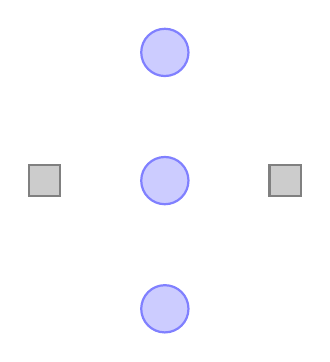
\begin{tikzpicture}
[place/.style={circle,draw=blue!50,fill=blue!20,thick,
inner sep=0pt,minimum size=6mm},
transition/.style={rectangle,draw=black!50,fill=black!20,thick,
inner sep=0pt,minimum size=4mm}]

\node[place] (waiting) {};
\node[place] (critical) [below=of waiting] {};
\node[place] (semaphore) [below=of critical] {};
\node[transition] (leave critical) [right=of critical] {};
\node[transition] (enter critical) [left=of critical] {};


\end{tikzpicture}

\end{document}
